\documentclass[11pt]{article}
\usepackage[letterpaper,margin=1in,headheight=14pt]{geometry}
\usepackage{amsmath,amssymb,amsthm}
\usepackage{booktabs}
\usepackage{array}
\usepackage{tikz}
\usepackage{enumitem}
\usepackage{microtype}
\usepackage[T1]{fontenc}
\usepackage{mathptmx}
\usepackage{titlesec}
\usepackage{fancyhdr}
\usepackage{framed}
\usepackage{xcolor}
\usetikzlibrary{arrows.meta,positioning,calc}

\definecolor{rule}{gray}{0.55}
\definecolor{shadecolor}{gray}{0.94}

\pagestyle{fancy}
\fancyhf{}
\fancyhead[L]{\small ECON 601 \textbullet\ Demand}
\fancyhead[R]{\small\thepage}
\renewcommand{\headrulewidth}{0.4pt}

\titleformat{\section}{\large\bfseries}{\thesection}{0.8em}{}
\titleformat{\subsection}{\normalsize\bfseries}{\thesubsection}{0.7em}{}
\titlespacing*{\section}{0pt}{16pt plus 3pt minus 2pt}{7pt}

\setlist[itemize]{leftmargin=1.3em,itemsep=2pt,topsep=4pt}
\setlist[enumerate]{leftmargin=1.5em,itemsep=3pt,topsep=4pt}

\newtheorem{theorem}{Theorem}
\newtheorem{proposition}{Proposition}
\newtheorem{lemma}{Lemma}
\theoremstyle{definition}
\newtheorem{definition}{Definition}

\newenvironment{keybox}{\begin{snugshade}\noindent\ignorespaces}{\end{snugshade}}

\newcommand{\R}{\mathbb{R}}
\newcommand{\Rn}{\mathbb{R}^n_+}
\newcommand{\pref}{\succsim}
\newcommand{\xs}{x^*}
\newcommand{\pdd}[2]{\frac{\partial #1}{\partial #2}}
\newcommand{\src}[1]{\textit{\small (#1)}}
\newcommand{\back}[1]{\textbf{\small $\leftarrow$ L1:} \small #1}
\newcommand{\fwd}[1]{\textbf{\small $\rightarrow$ L3:} \small #1}

\begin{document}

\begin{center}
{\LARGE\bfseries Demand}\\[5pt]
{\large ECON 601, Lecture 2 in context}\\[9pt]
{\small What Lecture 1 hands over, what Lecture 2 does with it, and where Lecture 3 takes it}
\end{center}

\vspace{6pt}\hrule\vspace{9pt}

{\small
\noindent\textbf{How this is organised.} Not section by section. The document follows the
four questions Lecture 2 asks, in the order it asks them. Lecture 1 material appears where
Lecture 2 needs it, flagged \back{like this}. Lecture 3 appears as the destination, flagged
\fwd{like this}. Page references point to the lecture PDFs; RS1--RS3 are the review session
solutions; J\&R is Jehle and Reny, 3rd edition.
}

\vspace{9pt}\hrule

\tableofcontents
\clearpage

%==================================================================
\section{Why any of this exists}
%==================================================================

Preferences are invisible. Nobody can observe a ranking inside someone's head, and no
survey recovers one reliably. Prices, incomes, and quantities purchased are visible, and
governments and firms collect them constantly.

The entire construction is a bridge between those two facts. Lecture 1 builds an
unobservable object, a utility function, from assumptions about an unobservable ranking.
Lecture 2 pushes that object through a budget constraint to produce something observable:
what the consumer buys. Lecture 3 then runs the bridge in the other direction, recovering
what the consumer buys from how their welfare responds to prices, with no need to know the
utility function at all.

\begin{center}
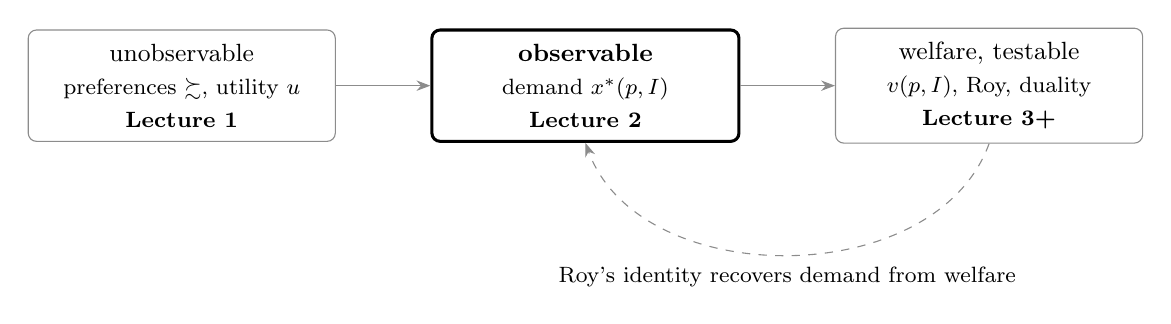
\begin{tikzpicture}[
  box/.style={draw=rule,rounded corners=3pt,align=center,inner sep=5pt,minimum width=3.9cm,font=\small},
  hi/.style={box,line width=1.1pt,draw=black},
  ar/.style={-{Stealth[length=5pt]},draw=rule}
]
\node[box] (a) at (0,0) {\small unobservable\\[1pt]\footnotesize preferences $\pref$, utility $u$\\[1pt]\footnotesize \textbf{Lecture 1}};
\node[hi,right=12mm of a] (b) {\small \textbf{observable}\\[1pt]\footnotesize demand $\xs(p,I)$\\[1pt]\footnotesize \textbf{Lecture 2}};
\node[box,right=12mm of b] (c) {\small welfare, testable\\[1pt]\footnotesize $v(p,I)$, Roy, duality\\[1pt]\footnotesize \textbf{Lecture 3+}};
\draw[ar] (a)--(b); \draw[ar] (b)--(c);
\draw[ar,dashed] (c.south) to[out=250,in=290] node[below,font=\footnotesize,yshift=-1pt] {Roy's identity recovers demand from welfare} (b.south);
\end{tikzpicture}
\end{center}

\vspace{4pt}
Lecture 2 is the middle of that bridge, which is why it carries most of the weight. It
answers four questions, and it answers them in this order for a reason: each question costs
one more assumption than the last.

\begin{center}
\begin{tabular}{@{}p{0.5cm}p{6.4cm}p{3.5cm}p{3.6cm}@{}}
\toprule
& \textbf{Question} & \textbf{Assumption it costs} & \textbf{Where answered} \\
\midrule
Q1 & Does a best affordable bundle exist at all? & continuity of $u$; $p\gg0$ & Section 3 \\[3pt]
Q2 & Is it one bundle or many? & curvature of $u$ & Section 4 \\[3pt]
Q3 & What is true of it no matter who the consumer is? & monotonicity & Section 5 \\[3pt]
Q4 & How do you actually compute it? & differentiability & Section 6 \\
\bottomrule
\end{tabular}
\end{center}

\vspace{5pt}
That ordering is the single most useful thing to carry. When a later step confuses you, the
question to ask is almost always: \emph{which assumption is this step spending?} The four
families are:

\begin{center}
\begin{tabular}{@{}p{2.9cm}p{4.0cm}p{7.4cm}@{}}
\toprule
\textbf{Family} & \textbf{Hypotheses} & \textbf{What it controls, and only this} \\
\midrule
Regularity & continuity of $u$, compactness of $B$ & whether the maximum is attained, and how the \emph{value} behaves \\[3pt]
Curvature & quasi-concavity, strict quasi-concavity & how many \emph{solutions}, and the shape of the solution set \\[3pt]
Monotonicity & $u$ strictly increasing in some good & \emph{where} the solution sits, in particular whether the budget binds \\[3pt]
Smoothness & differentiability & whether calculus is available \\
\bottomrule
\end{tabular}
\end{center}

\begin{keybox}
\textbf{The mistake this prevents.} Expecting a claim to deliver something from a different
family. Continuity buys existence and says nothing about uniqueness. Strict quasi-concavity
buys uniqueness and says nothing about whether income is spent. Both errors are common and
both are avoided by naming the family first.
\end{keybox}

\clearpage

%==================================================================
\section{What Lecture 1 hands over}
%==================================================================

Lecture 1 is not a separate subject. It is the supplier. Everything in it that Lecture 2
uses fits on this page; the rest is background you can leave until revision.

\subsection{The delivery manifest}

\begin{center}
\begin{tabular}{@{}p{4.2cm}p{4.1cm}p{6.0cm}@{}}
\toprule
\textbf{Lecture 1 gives} & \textbf{Becomes} & \textbf{Used in Lecture 2 for} \\
\midrule
A1, A2 completeness and transitivity & a ranking & the problem being well posed at all \\[3pt]
A3 continuity & a continuous $u$ (Debreu) & \textbf{Q1}: existence of $\xs$ \\[3pt]
A4 monotonicity & $u$ increasing & \textbf{Q3}: the budget binds \\[3pt]
A5 convexity & $u$ quasi-concave & \textbf{Q2}: the solution set is convex \\[3pt]
A5$'$ strict convexity & $u$ strictly quasi-concave & \textbf{Q2}: the solution is unique \\[3pt]
$X$ closed, convex, $0\in X$ \src{RS1 Q1.2} & properties of the domain & \textbf{Q1}: $B$ is closed and convex \\[3pt]
Prop 1.1 invariance & $u$ is ordinal & \textbf{Q4}: a check on every answer \\[3pt]
MRS and its invariance & the right marginal object & \textbf{Q4}: the tangency condition \\
\bottomrule
\end{tabular}
\end{center}

\subsection{Two facts from Lecture 1 that shape every answer}

\paragraph{Utility is ordinal \src{L1 Prop 1.1, p.6}.} If $u$ represents $\pref$ and $h$ is
strictly increasing, then $h[u]$ represents the same preferences. So infinitely many utility
functions describe one consumer.

This is not philosophy; it is a working constraint. Any feature of your demand answer that
depends on which representation you picked is an \emph{error}. When a multiplicative
constant survives into your demand function, you have made a mistake, and you know it
without rechecking a line of algebra.

\paragraph{Marginal utility is the wrong primitive; MRS is the right one \src{L1 p.17}.}
Replacing $u$ by $1000u$ multiplies every marginal utility by $1000$. Marginal utility is
therefore meaningless on its own. The ratio survives, because the scaling cancels:
\[
MRS_{2,1}\Big|_{u_0}=\frac{\partial u/\partial x_1}{\partial u/\partial x_2}
=\left|\frac{dx_2}{dx_1}\right|_{u_0},
\]
and L1 p.19 confirms $u$ and $h[u]$ share it. This is exactly why the optimality condition
in Lecture 2 is written as an MRS equalling a price ratio and not as marginal utilities
equalling anything. The theory is built out of the objects that survive the ordinality
problem.

\subsection{Quasi-concavity, since Q2 runs on it}

\begin{definition}[L1 Def 1.3, p.13]
$f$ is quasi-concave if for all $x^1,x^2$ and $t\in[0,1]$,
$f(tx^1+(1-t)x^2)\ge\min\{f(x^1),f(x^2)\}$, and strictly quasi-concave if the inequality is
strict for $x^1\ne x^2$, $t\in(0,1)$.
\end{definition}

RS2 Q1.1 derives this definition instead of asserting it. Start from convex preferences,
take $x^1\succ x^2$, note that the better-than set of $x^2$ is convex so the combination
lies in it, and translate back through the definition of $u$. The $\min$ appears because
$u(x^2)$ is the smaller of the two values. Equivalently \src{L1 Thm 1.2}, $f$ is
quasi-concave exactly when every better-than set $\{x: f(x)\ge K\}$ is convex.

\begin{keybox}
\textbf{Trap.} Diminishing MRS in every pair does \emph{not} give quasi-concavity once
there are more than two goods. Counterexample \src{RS2 Ex 1.3}: for
$u(x)=x_1+(x_2x_3)^{2/3}$, the bundles $(16,0,0)$ and $(0,8,8)$ are both worth $16$, while
the combination $(14,1,1)$ is worth $15$. L1 Proposition 1.5 states the equivalence for two
goods only.
\end{keybox}

\subsection{The four special functions are the four cases}

These are one family, CES, at three limits \src{L1 pp.19--20; the Cobb-Douglas limit is
proved in RS2 Q2.2}. They are in the course because between them they exhaust the answers
Lecture 2 can give.

\begin{center}
\begin{tabular}{@{}p{2.7cm}p{3.3cm}p{3.2cm}p{5.0cm}@{}}
\toprule
\textbf{Function} & \textbf{Curvature} & \textbf{Answer to Q2} & \textbf{Why it is in the course} \\
\midrule
Cobb-Douglas & strictly quasi-concave & unique, interior & the case where every theorem applies \\[3pt]
Linear & quasi-concave, not strictly & multiple, or a corner & breaks uniqueness; breaks continuity of demand in L3 \\[3pt]
Leontief & quasi-concave, not strictly & unique, at the kink & shows strictness is sufficient, not necessary \\[3pt]
Max \src{L1 p.20} & not quasi-concave & extremes preferred & non-convex preferences, the RS1 Q1.6 trip \\
\bottomrule
\end{tabular}
\end{center}

\vspace{3pt}
The Leontief row is the one people miss. Its solution is unique despite failing strict
quasi-concavity, which proves the Lecture 2 uniqueness result is a one-way implication. It
is also the case where calculus fails outright, since there is no derivative at the kink.

\vspace{4pt}
\noindent\textit{Background you can defer:} Debreu's theorem and its proof, lexicographic
preferences, the countability argument, and the concave-versus-quasi-concave examples. None
of it is used by Lecture 2. Read it when the axioms-to-utility step starts to feel like a
black box.

\clearpage

%==================================================================
\section{Q1: does a best affordable bundle exist?}
%==================================================================

\subsection{Why the question is not trivial}

It is easy to write down a maximisation and assume it has an answer. It need not. Two
things can go wrong. The consumer might improve forever without arriving, which happens
when the feasible set is unbounded. Or the objective might jump, so the supremum is
approached but never reached.

Ruling both out is the job of this section, and everything after it silently assumes the
job was done.

\subsection{The budget set}

Lecture 1 gave preferences but no scarcity: everything in $X$ was imaginable. Scarcity
enters here. In two goods, $B$ is the triangle with corners at the origin, $(I/p_1,0)$ and
$(0,I/p_2)$.

\begin{definition}[L2 p.2]
$B=\{x\in X: p\cdot x\le I\}$, with $p\gg0$ and $I>0$.
\end{definition}

\begin{proposition}[L2 p.2, left as an exercise]
$B$ is nonempty, convex and compact.
\end{proposition}

\paragraph{Proof.} \emph{Nonempty:} the origin lies in $X=\Rn$ and costs nothing, and
$I>0$. \back{$0\in X$ is one of the standing assumptions on the consumption set, RS1 Q1.2.}

\emph{Convex:} take $x^1,x^2\in B$ and $t\in[0,1]$. The combination stays in $X$ because
$X$ is convex. By linearity of the dot product,
\[
p\cdot\big(tx^1+(1-t)x^2\big)=t\,(p\cdot x^1)+(1-t)\,(p\cdot x^2)\le tI+(1-t)I=I.
\]

\emph{Closed:} $g(x)=p\cdot x$ is continuous and $B=X\cap g^{-1}((-\infty,I])$. The preimage
of a closed set under a continuous map is closed, $X$ is closed, and intersections of closed
sets are closed.

\emph{Bounded:} fix $i$. Every term in the expenditure sum is nonnegative, so one term is no
larger than the whole:
\[
p_ix_i\le \sum_j p_jx_j = p\cdot x\le I
\qquad\Longrightarrow\qquad
0\le x_i\le \frac{I}{p_i}.
\]
So $B$ sits inside the box $\prod_i[0,I/p_i]$. Closed and bounded gives compact. \hfill$\square$

\subsection{Why that settles the question}

Lecture 2, p.2 lists three facts about compactness without naming the theorem they amount
to. Together they are Weierstrass: a continuous function on a compact set attains its
maximum. Compactness of $B$ stops the consumer escaping to infinity; continuity of $u$
stops the maximum falling through a gap.

\begin{definition}[UMP and Marshallian demand, L2 p.2]
\[
\max_{x\in\Rn} u(x)\quad\text{s.t.}\quad p\cdot x\le I,
\qquad\text{solution } \xs(p,I).
\]
\end{definition}

\subsection{Which hypothesis did what}

The convexity half of the proof used nothing about prices. The boundedness half used
$p\gg0$, and only there, to divide by $p_i$.

So if some $p_i=0$, then $B$ stays nonempty, convex and closed, but $x_i$ is unbounded. $B$
is no longer compact, Weierstrass no longer applies, and if $u$ is strictly increasing in
good $i$ the UMP has \emph{no solution at all}. This is the cleanest example in the course
of one hypothesis doing exactly one job.

\begin{keybox}
\fwd{Indirect utility is defined as the maximised value, $v(p,I)=u(\xs(p,I))$. That
definition is only meaningful because the maximum is attained. Lecture 3 never revisits
this; it simply assumes Q1 was answered.}
\end{keybox}

\vspace{4pt}
\noindent\textbf{Carry the convexity result forward.} The three-line convexity argument
above gets reused verbatim three more times: in the uniqueness proof (Section 4), in the
convex-solution-set proof (Section 4), and in the quasi-convexity proof of Lecture 3. In all
four the move is identical: scale two inequalities by weights summing to one, add, and
recognise the result.

\clearpage

%==================================================================
\section{Q2: is the answer one bundle or many?}
%==================================================================

\subsection{Why existence did not settle this}

These are different questions and they are secured by different features.

Existence asks whether the best value is reached, and is settled by regularity. Uniqueness
asks whether that value is reached at one point or several, and regularity has nothing to
say about it. Continuity restricts local jumps; it places no restriction at all on whether
two distant bundles tie. A constant function is perfectly continuous and every point
maximises it.

\begin{center}
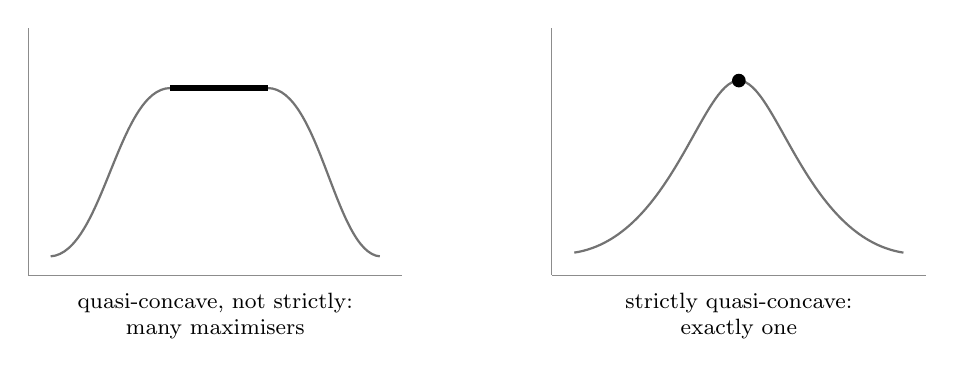
\begin{tikzpicture}[scale=0.95]
\begin{scope}
\draw[draw=rule] (0,0)--(5,0);
\draw[draw=rule] (0,0)--(0,3.3);
\draw[thick,draw=black!55] (0.3,0.25) .. controls (1.0,0.3) and (1.2,2.5) .. (1.9,2.5)
   -- (3.2,2.5) .. controls (3.9,2.5) and (4.1,0.3) .. (4.7,0.25);
\draw[line width=2pt] (1.9,2.5)--(3.2,2.5);
\node[font=\footnotesize,align=center] at (2.5,-0.55) {quasi-concave, not strictly:\\ many maximisers};
\end{scope}
\begin{scope}[xshift=7cm]
\draw[draw=rule] (0,0)--(5,0);
\draw[draw=rule] (0,0)--(0,3.3);
\draw[thick,draw=black!55] (0.3,0.3) .. controls (1.6,0.5) and (2.0,2.6) .. (2.5,2.6)
   .. controls (3.0,2.6) and (3.4,0.5) .. (4.7,0.3);
\fill (2.5,2.6) circle (2.6pt);
\node[font=\footnotesize,align=center] at (2.5,-0.55) {strictly quasi-concave:\\ exactly one};
\end{scope}
\end{tikzpicture}
\end{center}

\vspace{4pt}
The lecture's own counterexample is on p.3: with $u=x_1+x_2$, $p_1=p_2=1$ and $I=10$, the
maximum is $10$ and every bundle on the budget line attains it. The figures on pp.3 and 4
are the two panels above, drawn as indifference curves.

\subsection{The two results, and the single character that separates them}

\begin{proposition}[L2 p.3; RS3 Q1.1]
If $u$ is strictly quasi-concave then $\xs$ is unique.
\end{proposition}

\paragraph{Proof.} Suppose distinct $x'^*$ and $x''^*$ both solve the UMP, so
$u(x'^*)=u(x''^*)$. Form $x^{t*}=tx'^*+(1-t)x''^*$ for $t\in(0,1)$. \back{Convexity of $B$
from Q1 makes this feasible.} Strict quasi-concavity gives
$u(x^{t*})>\min\{u(x'^*),u(x''^*)\}=u(x'^*)$, contradicting optimality. \hfill$\square$

\begin{proposition}[L2 p.6]
If $u$ is quasi-concave then the set of solutions is convex.
\end{proposition}

\paragraph{Proof.} Let $v$ be the maximised value and take two solutions. The combination
is feasible by the same appeal to convexity of $B$, and quasi-concavity gives
$u(\xs)\ge\min\{\cdot,\cdot\}=v$. But $v$ is the maximum over $B$, so $u(\xs)\le v$ too.
Hence $u(\xs)=v$ and the combination is itself a solution. \hfill$\square$

\begin{keybox}
\textbf{Read the two proofs side by side.} Same setup, same combination, same appeal to
convexity of $B$. The only difference is whether the key inequality is strict. Strict
produces a contradiction, so the second solution cannot exist. Weak produces no
contradiction and instead proves membership. One character flips the conclusion from
``exactly one'' to ``possibly many, forming a convex set.''
\end{keybox}

\vspace{4pt}
\noindent\textbf{Sufficient, not necessary.} \back{Leontief preferences are not strictly
quasi-concave, yet the UMP solution is unique, at the kink.} The proposition is a one-way
implication. Failing its hypothesis tells you nothing.

\subsection{The mirror-image error}

Having just learned that strictness buys uniqueness, it is tempting to think it buys
tidiness in general. It does not. Take the bliss-point utility
\[
u(x,y)=-(x-x_0)^2-(y-y_0)^2,\qquad I>p_xx_0+p_yy_0.
\]
This is strictly quasi-concave, so the solution is unique, and continuous, so it exists.
And the consumer leaves income unspent \src{RS2 Q2.3}. Uniqueness bought one solution and
said nothing about \emph{where} that solution sits. That is Q3's job.

\begin{keybox}
\fwd{The same split appears one level up. Continuity of $u$ gives continuity of $v$ but not
of $\xs$; Proposition 3.1 needs strict quasi-concavity for demand to be continuous \src{L3
p.5}. Regularity governs the value, strictness governs the solution. With linear utility,
$v=I/\min\{p_1,p_2\}$ glides smoothly while demand jumps from one axis to the other. Same
logic, same counterexample, one lecture later.}
\end{keybox}

\clearpage

%==================================================================
\section{Q3: what is true regardless of who the consumer is?}
%==================================================================

\subsection{Why this is the section that matters empirically}

Q1 and Q2 are housekeeping: they establish that the object exists and is well defined. They
say nothing you could take to data, because they are statements about the model.

This section is different. Both results here hold for \emph{every} consumer satisfying the
axioms, whatever their tastes. That makes them the only claims so far that could be
falsified by observing actual purchases, and it is why they are the empirical content of
consumer theory.

\subsection{Property 1: demand is HD0 in $(p,I)$}

\[
\xs(tp,tI)=t^0\,\xs(p,I)=\xs(p,I)\qquad\text{for all } t>0
\]

\paragraph{Why it must be true.} Demand cannot see prices and income at all. It can only
see the budget set. And scaling every price and income by the same factor draws the
\emph{identical} triangle, not a similar one. The consumer is solving a problem already
solved.

Formally \src{L2 p.5}, the objective $u(x)$ contains no prices or income, and the scaled
constraint $tp\cdot x\le tI$ divides by $t$ back into the original. Same objective over the
same feasible set gives the same solution. The proof needs nothing about the consumer,
which is exactly the point.

\paragraph{Intuition.} Scaling a triangle changes its side lengths but not its angles.
Lengths are degree one, angles are degree zero. Demand is an angle. The concrete version is
a currency redenomination: a country drops three zeros, a coffee goes from $5{,}000$ to
$5$ and your salary from $4{,}000{,}000$ to $4{,}000$, and you buy the same coffee.

\paragraph{Three uses.}
\begin{enumerate}
\item \emph{It removes a variable.} Choosing $t=1/I$ gives $\xs(p,I)=\xs(p/I,1)$, so demand
really depends on $n$ numbers, prices measured in units of income. This is why general
equilibrium normalises prices, and why only relative prices are ever determined.
\item \emph{It is a free error check.} Scale your final expression and confirm the scaling
cancels. This is the economist's version of checking units, and it catches algebra errors
in seconds.
\item \emph{It is a restriction you can estimate.} See the elasticity form below.
\end{enumerate}

\paragraph{It is an assumption, not a tautology.} HD0 is the formal statement that this
consumer has no money illusion. Real people demonstrably respond to nominal magnitudes:
they resist nominal wage cuts while accepting real cuts delivered by inflation, and they
anchor on remembered nominal prices. The model was built to have this property. Knowing
which step delivers it, the line where $t$ divides out of the budget constraint, is what
lets you say something sensible when model and behaviour disagree.

\subsection{The detour Lecture 2 takes here, and why}

To turn HD0 into a statement about derivatives, the lecture stops and introduces
homogeneous functions \src{L2 pp.4--5}. This looks like a digression and is not.

\begin{definition}[L2 Def 2.1]
$f$ is homogeneous of degree $k$ if $f(tx)=t^kf(x)$ for all $x$ and all $t>0$.
\end{definition}

The crucial remark, made explicitly in RS3, is that this is an \emph{identity}: it holds for
every $x$ and every $t$, so it may be differentiated with respect to either. Most people
read the definition as a test to apply and never notice it is an equation to manipulate.

\begin{theorem}[Euler, L2 Thm 2.1]
For differentiable $f$, $f$ is homogeneous of degree $k$ if and only if
$\sum_i \pdd{f}{x_i}x_i = k f(x)$ for all $x$.
\end{theorem}

\paragraph{Why it is true, geometrically.} Walk outward along the ray through a bundle and
record the value, $g(t)=f(tx)$. Homogeneity says that along every such ray $f$ is an
ordinary power function. Differentiating that one-variable function two ways, directly and
by the chain rule, and evaluating at $t=1$, gives the theorem. The left side is the rate of
change of $f$ as you move radially outward from the origin; Euler says that radial rate is
pinned down by the value and the degree, and nothing else.

\paragraph{What Euler is for.} Homogeneity is a global claim about every scaling at once,
which is awkward to check and impossible to differentiate. Calculus is local. Euler is the
bridge between them, converting a global scaling property into one equation holding at each
point, involving nothing but first derivatives.

\paragraph{The payoff, immediately.} Apply it to demand with $k=0$, remembering the
arguments are the $n$ prices \emph{and} income:
\[
\pdd{x_i^*}{p_1}p_1+\cdots+\pdd{x_i^*}{p_n}p_n+\pdd{x_i^*}{I}I=0
\qquad\Longleftrightarrow\qquad
\sum_j \varepsilon_{ij}+\eta_i=0.
\]
In words: all the price elasticities for good $i$ and its income elasticity sum to exactly
zero. Estimate a demand system on real data and you can test that. A definitional property
became a falsifiable one, and Euler is what did it.

\begin{keybox}
\textbf{Trap.} Always check \emph{which} variables the homogeneity is in before writing the
Euler sum. Demand is homogeneous in prices and income together, so the sum has $n+1$ terms.
A utility function homogeneous in quantities gives $n$ terms. Wrong count is the most common
error with this theorem.
\end{keybox}

\vspace{3pt}
\noindent The companion result \src{RS3 Prop 1} is that $\partial f/\partial x_i$ is
homogeneous of degree $k-1$. That is the bookkeeping which keeps the degrees consistent
across the course.

\begin{center}
\begin{tabular}{@{}lcll@{}}
\toprule
\textbf{Object} & \textbf{Degree} & \textbf{In} & \textbf{Where} \\
\midrule
Marshallian demand & 0 & prices and income & L2 \\
Indirect utility & 0 & prices and income & L3 \\
Expenditure function & 1 & prices & next \\
Hicksian demand & 0 & prices & next \\
Cost, profit functions & 1 & input prices & later in the sequence \\
\bottomrule
\end{tabular}
\end{center}

\subsection{Property 2: the budget binds}

\begin{proposition}[L2 p.6; RS3 Q3.2(b)]
If $u$ is strictly increasing in some $x_i$, then $p\cdot\xs=I$.
\end{proposition}

\back{This is Axiom 4 cashing in. Monotonicity was introduced in Lecture 1 with the remark
that it would ``later ensure the use of one's income.'' This is later.}

\paragraph{Proof.} Suppose not. Any solution is feasible, so failure means
$p\cdot\xs<I$. Let good $i$ be one in which $u$ is strictly increasing, and set
\[
\delta = I-p\cdot\xs>0,\qquad \varepsilon=\frac{\delta}{p_i}>0,
\]
the division being legitimate because $p\gg0$. Construct
$\bar x=(x_1^*,\dots,x_i^*+\varepsilon,\dots,x_n^*)$. It is nonnegative, and
\[
p\cdot\bar x = p\cdot\xs+p_i\varepsilon = p\cdot\xs+\delta = I,
\]
so it is feasible. Since $u$ is strictly increasing in good $i$ and only that component
rose, $u(\bar x)>u(\xs)$, contradicting optimality. \hfill$\square$

\vspace{3pt}
\noindent Two remarks. The lecture says ``increase $x$ by $\varepsilon$'' without
specifying $\varepsilon$; choosing the one that exactly exhausts the slack makes
feasibility an equality instead of an estimate. And the hypothesis is deliberately weak:
strictly increasing in \emph{some} good, not all. You only need one good worth buying more
of.

\paragraph{Why it is needed.} Without it the first-order conditions give you ratios and
nothing else. The binding budget is the extra equation that converts a ratio into
quantities, which is why every worked example in Section 6 deduces it before solving.

\begin{keybox}
\fwd{In Lecture 3 this result is what makes $\partial v/\partial I=\lambda^*>0$. Roy's
identity divides by that derivative, so the strict positivity is load-bearing, not
decoration. It also signs $\partial v/\partial p_i=-\lambda^*x_i^*<0$. Further ahead, the
mirror result in expenditure minimisation, that the utility constraint binds, is what makes
duality close.}
\end{keybox}

\clearpage

%==================================================================
\section{Q4: how do you compute it?}
%==================================================================

\subsection{The problem ordinary calculus cannot handle}

Calculus finds a maximum by setting derivatives to zero, which works because at the top of
an unconstrained hill the ground is flat. Consumer problems break this. The unconstrained
peak of a utility function is at infinite consumption. The point you actually reach sits on
the edge of the budget set, and there the derivative of utility is emphatically not zero.
You are still going uphill; you have run out of money.

Everything in this section is machinery for getting calculus back.

\subsection{The Lagrangian}

\begin{definition}[L2 p.7]
\[
\mathcal{L}(x,\lambda)=u(x)+\lambda\,[\,I-p\cdot x\,],
\qquad
\max_x\min_\lambda \mathcal{L}\ \ \text{s.t. } x\ge0,\ \lambda\ge0.
\]
\end{definition}

The bracket is leftover income: zero on the budget line, positive inside the budget set,
negative if you overspend. Read $\lambda$ as a price on money. Every dollar left over is
credited at rate $\lambda$, every dollar of overspending charged at rate $\lambda$. You are
now free to buy anything at all, because overspending is priced instead of forbidden. The
constraint has been folded into the objective.

\paragraph{Why max then min.} The inner minimisation is what enforces the constraint.
Propose an unaffordable bundle: the bracket is negative, so minimising over $\lambda\ge0$
drives $\lambda$ up without bound and the expression to $-\infty$. Cheating is made
infinitely unattractive. Propose a bundle with money left over: the bracket is positive, so
the minimisation sets $\lambda=0$, killing the term and leaving plain utility. The penalty
is thus set automatically at exactly the right severity, which is why the figure on p.7
shows a saddle point.

\paragraph{The geometry.} Setting the quantity derivatives to zero gives
$\nabla u(\xs)=\lambda^*p$. The gradient is the direction of steepest increase in utility;
$p$ is perpendicular to the budget line. So at the optimum, uphill points straight out of
the budget set. That is precisely the condition for being stuck: if the gradient had any
component running \emph{along} the budget line you could slide that way, stay affordable,
and gain. The multiplier is only the proportionality constant between two vectors that
turned out to be parallel.

\begin{center}
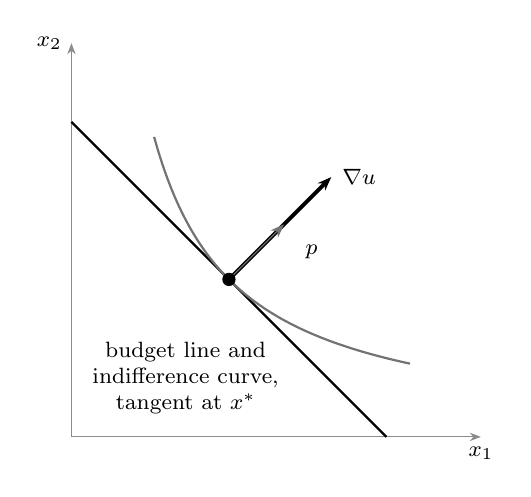
\begin{tikzpicture}[scale=1.0]
\draw[draw=rule,-{Stealth[length=4pt]}] (0,0)--(5.2,0) node[below,font=\footnotesize] {$x_1$};
\draw[draw=rule,-{Stealth[length=4pt]}] (0,0)--(0,5.0) node[left,font=\footnotesize] {$x_2$};
\draw[thick] (0,4)--(4,0);
\draw[thick,draw=black!55,domain=1.05:4.3,samples=80,smooth] plot (\x,{4/\x});
\draw[-{Stealth[length=5pt]},line width=1.4pt] (2,2)--(3.3,3.3) node[right,font=\footnotesize] {$\nabla u$};
\draw[-{Stealth[length=5pt]},draw=black!55] (2,2)--(2.7,2.7);
\node[font=\footnotesize] at (3.05,2.35) {$p$};
\fill (2,2) circle (2.4pt);
\node[font=\footnotesize,align=center] at (1.45,0.75) {budget line and\\ indifference curve,\\ tangent at $x^*$};
\end{tikzpicture}
\end{center}

\subsection{Kuhn-Tucker, built from one variable}

The conditions on p.7 look forbidding. They are one idea from single-variable calculus,
repeated once per good. Strip away utility, prices and vectors.

\paragraph{Step 1: maximising when the variable cannot go negative.} Consider
$\max_x f(x)$ subject to $x\ge0$. Two things can happen, and they are the two pictures on
L2 p.8.

\begin{center}
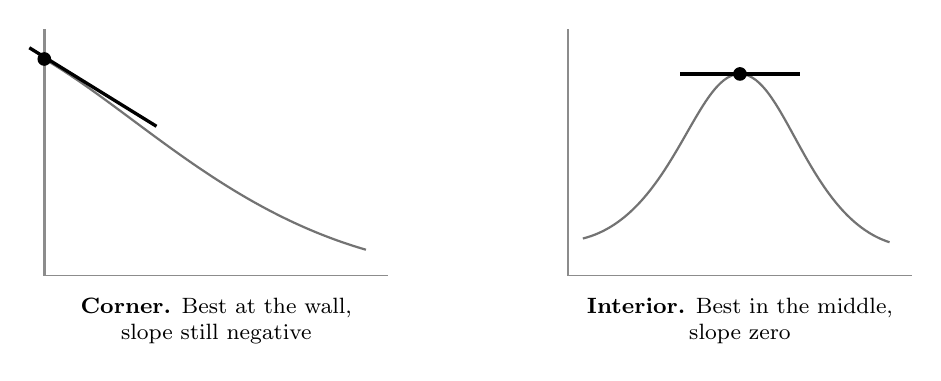
\begin{tikzpicture}[scale=0.95]
\begin{scope}
\draw[draw=rule] (0,0)--(4.6,0);
\draw[draw=rule,line width=1pt] (0,0)--(0,3.3);
\draw[thick,draw=black!55] (0,2.9) .. controls (1.2,2.2) and (2.4,0.9) .. (4.3,0.35);
\draw[line width=1.2pt] (-0.2,3.05)--(1.5,2.0);
\fill (0,2.9) circle (2.6pt);
\node[font=\footnotesize,align=center] at (2.3,-0.6) {\textbf{Corner.} Best at the wall,\\ slope still negative};
\end{scope}
\begin{scope}[xshift=7cm]
\draw[draw=rule] (0,0)--(4.6,0);
\draw[draw=rule,line width=1pt] (0,0)--(0,3.3);
\draw[thick,draw=black!55] (0.2,0.5) .. controls (1.4,0.8) and (1.7,2.7) .. (2.3,2.7)
  .. controls (2.9,2.7) and (3.2,0.8) .. (4.3,0.45);
\draw[line width=1.2pt] (1.5,2.7)--(3.1,2.7);
\fill (2.3,2.7) circle (2.6pt);
\node[font=\footnotesize,align=center] at (2.3,-0.6) {\textbf{Interior.} Best in the middle,\\ slope zero};
\end{scope}
\end{tikzpicture}
\end{center}

\vspace{6pt}
For $f(x)=10x-x^2$ the peak is at five and the slope there is zero. For $f(x)=-3x-x^2$ the
slope at zero is $-3$ and only worsens, so the best you can do is sit at zero, and the slope
at the optimum is \emph{not} zero. You would love to move left and climb, but negative
quantities are forbidden. You are pinned against a wall.

\paragraph{Step 2: one statement covering both.} Could the slope at the optimum be positive?
No: you could then step right, stay legal, and do better. That rules out one of three
possibilities and leaves two, which is the first line: $f'(x^*)\le0$. Strictly negative
means pinned at the wall; zero means a genuine hilltop.

\paragraph{Step 3: the product is an ``or'' written as an equation.} Either the quantity is
zero or the slope is zero. Two numbers multiply to zero exactly when one of them is zero, so
that ``or'' compresses to $f'(x^*)\cdot x^*=0$. That is all complementary slackness is. In
the first example the quantity is five and the slope is zero; in the second the quantity is
zero and the slope is $-3$. Both satisfy it, and nothing else does.

\paragraph{Step 4: put $\mathcal{L}$ in the role of $f$.} Holding $\lambda$ fixed, the
consumer's problem is exactly this shape with several quantities instead of one. Apply
Steps 2 and 3 good by good.

\begin{definition}[Kuhn-Tucker conditions, L2 p.7]
\begin{align*}
\pdd{\mathcal{L}}{x_i}&=\pdd{u}{x_i}-\lambda p_i\le 0, & \pdd{\mathcal{L}}{x_i}\,x_i^*&=0,\\[2pt]
\pdd{\mathcal{L}}{\lambda}&=I-p\cdot \xs\ge 0, & \pdd{\mathcal{L}}{\lambda}\,\lambda^*&=0,\\[2pt]
\xs&\ge 0, & \lambda^*&\ge 0.
\end{align*}
\end{definition}

\paragraph{Step 5: the multiplier line is the same idea, flipped.} The multiplier also
cannot go negative, but $\mathcal{L}$ is \emph{minimised} over it, so both signs flip. Its
derivative is leftover income, so the inequality is only the budget constraint reappearing,
and the product is again an ``or'': either there is no leftover, so the budget binds, or the
multiplier is zero, so an extra dollar is worth nothing.

\begin{center}
\begin{tabular}{@{}p{6.4cm}p{7.8cm}@{}}
\toprule
\textbf{Line in the notes} & \textbf{What it says} \\
\midrule
derivative in good $i$ at most zero & you never leave a good where buying more would help \\
that derivative times the quantity is zero & either you buy none of good $i$, or it is exactly worth its price \\
leftover income at least zero & you did not overspend \\
leftover times the multiplier is zero & either you spend everything, or money is worthless to you \\
quantities and multiplier at least zero & you cannot buy negative amounts, and the penalty is not a subsidy \\
\bottomrule
\end{tabular}
\end{center}

\paragraph{Step 6: watch it work.} Take the quasi-linear example on L2 p.9,
$u=x_1+\ln x_2$, with both prices one. With $I=10$ the answer is $x_1^*=9$, $x_2^*=1$,
$\lambda^*=1$: both first-order conditions hold with equality, both quantities are positive,
leftover is zero. Now drop income to $1/2$. The answer becomes $x_1^*=0$, $x_2^*=1/2$,
$\lambda^*=2$, and
\[
\pdd{u}{x_1}-\lambda p_1 = 1-2 = -1<0,\qquad x_1^*=0,
\]
so the product is still zero. Good one is not worth its price at this income, so you buy
none and sit pinned at the wall with a negative slope. Setting that derivative equal to
zero, as ordinary calculus suggests, would have produced a negative quantity and a wrong
answer. That case is the whole reason the apparatus exists.

\subsection{Tangency}

If $x_i^*>0$ and $x_j^*>0$, both conditions hold with equality and dividing cancels
$\lambda^*$:
\[
\underbrace{\frac{\partial u/\partial x_i}{\partial u/\partial x_j}}_{MRS_{j,i}}
=\underbrace{\frac{p_i}{p_j}}_{\text{price ratio}}.
\]
\back{This is why Lecture 1 built the theory on MRS. Marginal utilities individually are
meaningless under monotone transformation; their ratio is invariant, so this equation says
something about the consumer and not about the arbitrary choice of $u$.}

The intuition on p.10 is the clearest sentence in the lecture. If $MRS_{j,i}=2$ while the
price ratio is one, you would privately trade one unit of $i$ for two of $j$ while the
market trades them one for one. You value $j$ less than everyone else does, so sell $j$ and
buy $i$ until the ratios meet.

Rearranged one good at a time, the same conditions read
$\big(\partial u/\partial x_i\big)/p_i=\lambda^*$: extra utility per dollar must be equal
across every good you buy, because otherwise you would move a dollar from the low-return
good to the high-return one. That common rate is what an extra dollar of income is worth,
which is why $\lambda^*$ is called the marginal utility of income.

\subsection{The whole apparatus on one function}

Cobb-Douglas is worth doing in full because it is the only one of the four special functions
that satisfies every hypothesis in the strict form, so every result from Q1 to Q4 applies at
once. \back{It is also not an arbitrary example: it is the CES family at the limit
$\rho\to0$, proved in RS2 Q2.2.}

\paragraph{Each axiom becomes a visible feature of the answer.}

\begin{center}
\begin{tabular}{@{}p{3.0cm}p{5.3cm}p{5.9cm}@{}}
\toprule
\textbf{From Lecture 1} & \textbf{Why Cobb-Douglas has it} & \textbf{What it produces in the answer} \\
\midrule
A1, A2 & free: comparing values of a real function inherits both from $\ge$ on $\R$ & the problem is well posed \\[3pt]
A3 continuity & $u$ continuous on $\Rn$ & \textbf{Q1}: a solution exists \\[3pt]
A5$'$ strict convexity & strictly quasi-concave; L1 p.15 verifies it for $xy$ via the hyperbola & \textbf{Q2}: the solution is unique \\[3pt]
A4 monotonicity & increasing in each good & \textbf{Q3}: the budget binds \\[3pt]
Prop 1.1 invariance & $A\cdot(\cdot)$ is a strictly increasing transformation & $A$ must vanish from the answer \\[3pt]
Prop 1.4 diminishing MRS & $MRS_{2,1}=\tfrac{\alpha}{1-\alpha}\tfrac{x_2}{x_1}$ & \textbf{Q4}: the tangency condition is valid \\
\bottomrule
\end{tabular}
\end{center}

\paragraph{The derivation \src{RS3 Q3.4}.} For $u=Ax_1^{\alpha}x_2^{1-\alpha}$, assume an
interior solution so both first-order conditions hold with equality. Dividing one by the
other removes $\lambda$ and $A$ at once and leaves the tangency condition, hence
\[
\frac{\alpha}{1-\alpha}\cdot\frac{x_2}{x_1}=\frac{p_1}{p_2}
\qquad\Longrightarrow\qquad
\frac{p_2x_2}{p_1x_1}=\frac{1-\alpha}{\alpha}.
\]
Now invoke Q3: the budget binds. Substituting gives $p_1x_1/\alpha=I$ and therefore
\[
x_1^*=\frac{\alpha I}{p_1},\qquad x_2^*=\frac{(1-\alpha)I}{p_2}.
\]

\paragraph{Why the exponents are expenditure shares.} The boxed display above is the reason,
and it is worth seeing that it has nothing to do with Cobb-Douglas being special. Tangency
forces the ratio of spending to equal the ratio of exponents; the binding budget then splits
income in exactly those proportions. The famous constant-share result is Lecture 1's MRS
meeting Lecture 2's tangency condition, and nothing more.

\paragraph{The audit, which is the real lesson.} Check the answer against Q1 to Q4 before
moving on.

\begin{enumerate}
\item Scale $(p,I)$ by $t$: the $t$ cancels top and bottom, confirming HD0.
\item Add up: $\alpha I+(1-\alpha)I=I$, confirming the budget binds.
\item The constant $A$ vanished, as ordinality requires. RS3 Q3.5 asks you to redo the whole
thing with $\ln u$ and verify identical demands.
\item Both quantities are strictly positive for any $p\gg0$ and $I>0$, so the interiority
assumption was self-consistent.
\end{enumerate}

Doing this is worth more under exam pressure than being fast, because it catches your own
algebra errors in seconds. It also gives you one function you know cold, so that later
general claims can be tested immediately. When a claim fails even for Cobb-Douglas it is
false; when it holds for Cobb-Douglas but you suspect strictness matters, linear utility is
the second thing to try.

\begin{keybox}
\fwd{The Lagrangian you just built is reused immediately, but differentiated with respect to
the \emph{parameters} instead of the quantities. That is the envelope theorem, and it
produces $\partial v/\partial I=\lambda^*$ and $\partial v/\partial p_i=-\lambda^*x_i^*$,
whose ratio is Roy's identity. Lecture 3 does not introduce new machinery here. It points
the same machinery in a different direction.}
\end{keybox}

\clearpage

%==================================================================
\section{Where this goes: Lecture 3 and beyond}
%==================================================================

\subsection{The move Lecture 3 makes}

Lecture 2 produced $\xs(p,I)$, a function from parameters to quantities. Lecture 3 asks a
different question about the same problem: not what you buy, but how well off you end up.

\begin{definition}[Indirect utility, L3 p.2]
$v(p,I)=u(\xs(p,I))$, the maximised value of the UMP.
\end{definition}

Why bother? Because $v$ is expressed entirely in observable, policy-relevant variables. RS3
puts it well: utility functions let you compare bundles conveniently, and indirect utility
lets you compare $(p,I)$ pairs conveniently. Taxes, subsidies, inflation and price shocks
are all changes in $(p,I)$, so $v$ is the object welfare analysis actually uses.

\subsection{What carries over, and what does not}

\begin{center}
\begin{tabular}{@{}p{4.6cm}p{4.6cm}p{5.0cm}@{}}
\toprule
\textbf{Property of $v$} & \textbf{Where it comes from} & \textbf{Same as demand?} \\
\midrule
HD0 in $(p,I)$ & the budget set is unchanged & yes, identical argument \\[3pt]
decreasing in $p_i$, increasing in $I$ & scaling the feasible set up or down & new \\[3pt]
quasi-convex in $(p,I)$ & budget-set containment & new, and the least obvious \\[3pt]
continuous in $(p,I)$ & Berge & value only, \emph{not} demand \\[3pt]
invariant to monotone transforms of $u$ & --- & \textbf{no}: demand is, $v$ is not \\
\bottomrule
\end{tabular}
\end{center}

\vspace{3pt}
That last row is a favourite exam target. For the same preferences, different
representations of $u$ give different $v$ values, though the ordering of those values is
unchanged.

\begin{keybox}
\textbf{The space trap.} Lecture 1 gave quasi-\emph{concavity} of $u$ over \emph{commodity}
space via \emph{better}-than sets. Lecture 3 gives quasi-\emph{convexity} of $v$ over
\emph{price-income} space via \emph{worse}-than sets. Same machinery, different object,
different space, opposite direction. And the result holds whether or not $u$ is
quasi-concave, because the proof never touches the shape of $u$: it shows
$B(p^t,I^t)\subseteq B(p^1,I^1)\cup B(p^2,I^2)$ using the same scale-and-add move you first
met proving $B$ convex in Section 3.
\end{keybox}

\subsection{The envelope theorem, which is the actual tool}

Everything above is description. This is the instrument, and it is what makes the rest of
the sequence cheap.

\paragraph{In one line.} When you are already at the top, moving does not help you, so you
may ignore the fact that you will move.

\paragraph{The picture.} Stand at the highest point on a hill and let someone tilt the
landscape. Your height changes for two reasons: the ground under your feet moved, and you
will shuffle to the new summit. But you were at the summit, so the ground around you was
flat, and shuffling buys almost nothing. To first order the new height is the old spot with
the ground moved under it. The indirect effect through re-optimising vanishes, because at
an optimum the slope is zero.

\paragraph{Where the name comes from.} Fix $x$ and ask what $f(x,a)$ does as $a$ changes:
one curve. Do that for every $x$ and you get a family. $M(a)=\max_x f(x,a)$ is the highest
one at each $a$, so it sits on top of the family and touches whichever curve is best there.
At the touching point the two are tangent, so their slopes agree. The slope of $M$ is what
you want; the slope of the fixed-$x$ curve is easy, because $x$ is not moving.

\begin{center}
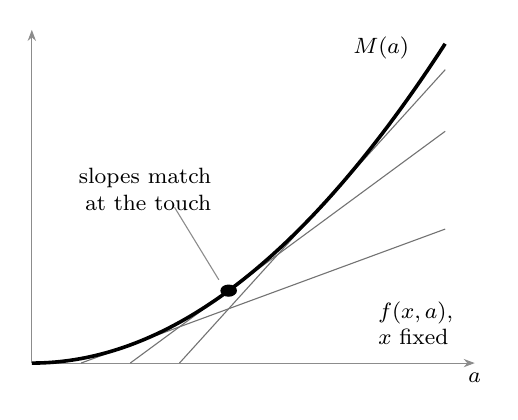
\begin{tikzpicture}[xscale=1.25,yscale=0.92]
\draw[draw=rule,-{Stealth[length=4pt]}] (0,0)--(4.5,0) node[below,font=\footnotesize] {$a$};
\draw[draw=rule,-{Stealth[length=4pt]}] (0,0)--(0,4.6);
\draw[draw=black!55] (0.5,0)--(4.2,1.85);
\draw[draw=black!55] (1.0,0)--(4.2,3.2);
\draw[draw=black!55] (1.5,0)--(4.2,4.05);
\draw[line width=1.3pt,domain=0:4.2,samples=90,smooth] plot (\x,{(\x)*(\x)/4});
\fill (2,1) circle (2.4pt);
\node[font=\footnotesize,align=right] at (1.15,2.4) {slopes match\\ at the touch};
\draw[draw=rule] (1.45,2.15)--(1.9,1.15);
\node[font=\footnotesize] at (3.55,4.35) {$M(a)$};
\node[font=\footnotesize,align=left] at (3.9,0.55) {$f(x,a)$,\\ $x$ fixed};
\end{tikzpicture}
\end{center}

\paragraph{Statement and check \src{L3 pp.5--7}.} The direct method gives
\[
M'(a)=\underbrace{f_x(x^*,a)}_{=\,0\text{ by the FOC}}\cdot x^{*\prime}(a)+f_a(x^*(a),a)
=f_a(x^*(a),a),
\]
so the envelope method skips to the end: differentiate $f$ with respect to $a$ treating $x$
as a parameter, then evaluate at $x^*(a)$. Test it on $f(x,a)=ax-x^2$. Directly,
$x^*(a)=a/2$, $M(a)=a^2/4$, $M'(a)=a/2$. By envelope, hold $x$ fixed and differentiate,
getting just $x$, then evaluate at $a/2$. Same answer, and $x^{*\prime}(a)$ was never
computed. Each straight line in the figure is this $f$ at fixed $x$ and its slope is that
$x$, so the slope of $M$ is simply the $x$ that is optimal there.

\back{You have already met the multiplier as the marginal value of a constraint: in the
small worked example of Section 6, $\lambda^*=5$ equalled $M'(10)$ exactly. That was the
envelope theorem before it was named.}

\subsection{Roy's identity, and why the sequence was built this way}

\begin{lemma}[L3 Lemma 3.1]
If $u$ is differentiable, strictly increasing and strictly quasi-concave, then
\[
x_i^*(p,I)=-\,\frac{\partial v/\partial p_i}{\partial v/\partial I}.
\]
\end{lemma}

\paragraph{Proof.} Write $v$ as the saddle value of the Lagrangian and apply the envelope
theorem to each parameter, holding $x$ and $\lambda$ fixed:
\[
\pdd{v}{I}=\lambda^*>0,
\qquad
\pdd{v}{p_i}=-\lambda^*x_i^*<0.
\]
Dividing cancels $\lambda^*$ and leaves $x_i^*$. \hfill$\square$

\vspace{3pt}
\noindent The entire content is that you were allowed to hold $\xs$ fixed while
differentiating. The direct method would require a chain-rule expansion across every good.
Note also which hypotheses are load-bearing: strict monotonicity is what makes the
denominator strictly positive, via the binding-budget result of Q3.

\paragraph{Why this closes the loop.} Return to Section 1. Utility is invisible; prices,
incomes and quantities are not. Roy's identity recovers what the consumer buys purely from
how their welfare responds to prices and income, with no knowledge of $u$. Every question
Lecture 2 answered was a step toward being able to write that formula down.

\subsection{What comes next}

Lecture 3 ends by noting that $\partial x_i^*/\partial p_i$ is complicated because several
effects are mixed together, and that an intermediate, more abstract problem is needed first.
That problem is expenditure minimisation, and it opens the second half of the chapter:

\begin{itemize}
\item the expenditure function $e(p,u)$ and Hicksian demand $h(p,u)$, the mirror images of
$v$ and $\xs$ \src{J\&R 1.4.2};
\item the duality relations tying all four objects together \src{J\&R 1.4.3};
\item the Slutsky decomposition into income and substitution effects, which is the answer to
the question Lecture 3 leaves hanging \src{J\&R 1.5.2};
\item elasticity relations, the fuller version of the restriction Euler gave you in Q3
\src{J\&R 1.5.3}.
\end{itemize}

The pattern to expect: the mirror problem has a mirror binding constraint, mirror
homogeneity degrees, and its own envelope result, Shephard's lemma, standing where Roy's
identity stands here.

\clearpage

%==================================================================
\section{Exercises, grouped by the question they answer}
%==================================================================

Four of the results proved above are left as ``Proof. Exercise.'' in the lecture notes.
Yildirim writes out the proofs he considers instructive to read and leaves the ones he
considers instructive to do, which makes them the closest thing to a stated exam preview
available. The proofs are in Sections 3 to 6; what follows is what each one is \emph{for}.

\subsection{On Q1}

\textbf{$B$ is nonempty, convex, compact \src{L2 p.2}.} The only result in Lecture 2 whose
failure would be invisible to you, since everything after p.2 silently assumes a solution
exists. It installs the cheapest and most-used skill in the course: write down what a
definition literally asserts and check it. Its convexity half is consumed three more times.

\emph{You have it when:} you can say which of the four properties fails if a price is zero,
and what goes wrong downstream.

\subsection{On Q2}

\textbf{Strict quasi-concavity gives uniqueness \src{L2 p.3; RS3 Q1.1; again as RS3
Q3.2(a)}.} Anything written out three times is not subtle signalling. It installs proof by
contradiction with a \emph{constructed witness}, which is where most people stall. The same
skeleton drives the quasi-convexity proof in Lecture 3.

\emph{You have it when:} you can state without looking which step uses convexity of $B$ and
which uses strictness.

\vspace{4pt}
\noindent\textbf{Quasi-concavity gives a convex solution set \src{L2 p.6}.} Low value alone,
high value as a contrast with the one above. Do it second, and read them side by side.

\emph{You have it when:} you can predict, before any algebra, which conclusion a weak
hypothesis will produce.

\vspace{4pt}
\noindent Also: RS3 Q3.3 (convex but not strictly: existence survives, uniqueness does not)
and RS2 Q1.1, Q1.2, Ex 1.3 on quasi-concavity itself. RS2 Ex 1.3 is the best single question
in the review sessions.

\subsection{On Q3}

\textbf{HD$k$ implies Euler \src{L2 p.4; RS3 Q1.2}.} The only pure technique on the list,
and the statement matters far less than the move: notice the definition is an identity, then
differentiate it. The payoff compounds, since degree zero gives the demand restriction and
degree one gives product exhaustion later in the sequence.

\emph{You have it when:} you can say why setting $t=1$ at the end is legitimate, and write
the Euler sum for demand with the right number of terms without counting.

\vspace{4pt}
\noindent\textbf{The budget binds \src{L2 p.6; RS3 Q3.2(b)}.} Read it with RS2 Q2.3, which
asks the true-or-false version and answers false using the bliss point. The pair shows
exactly which assumption carries the result. Add RS3 Q3.6 ($u=x_1$) for the corner case.

\subsection{On Q4}

\textbf{Cobb-Douglas, then the log transform \src{RS3 Q3.4, Q3.5}.} The derivation is not
the reason; the audit is. And it gives you one function you know cold to test later claims
against.

\emph{You have it when:} you can derive the demands without writing the Lagrangian, going
straight from tangency plus a binding budget.

\subsection{If you only work six}

RS2 Q1.1, RS2 Ex 1.3, RS3 Q1.1, RS3 Q1.2, the RS2 Q2.3 with RS3 Q3.2(b) pair, and RS3 Q3.4
with Q3.5. That covers axiom-to-function translation, the main counterexample, uniqueness,
the Euler technique, what makes the budget bind, and ordinality.

\subsection{Beyond the review sessions}

The review sessions work textbook problems and label them: RS1 Q1.2--Q1.6 are J\&R
Exercises 1.1--1.6, and RS3 Q3.1--Q3.6 are Exercises 1.12, 1.16, 1.17, 1.20, 1.21 and 1.26.
They cover roughly a third of Section 1.6. The rest are the same type, on the same material,
from the same source your TAs draw from, without posted solutions. On Lectures 1 and 2:
Exercises 1.5, 1.7, 1.8, 1.9, 1.10 and 1.13--1.15. Exercise 1.7 is the direct companion to
the two Q2 proofs.

\clearpage

%==================================================================
\section{Reference card}
%==================================================================

\subsection{The four questions and their answers}

\begin{center}
\begin{tabular}{@{}p{0.6cm}p{4.3cm}p{4.4cm}p{4.7cm}@{}}
\toprule
& \textbf{Question} & \textbf{Answer} & \textbf{Needs} \\
\midrule
Q1 & does $\xs$ exist? & yes & $u$ continuous, $B$ compact, so $p\gg0$ \\[3pt]
Q2 & is it unique? & yes if strictly quasi-concave; otherwise the solution set is convex & curvature \\[3pt]
Q3 & what always holds? & HD0 in $(p,I)$; $p\cdot\xs=I$ & monotonicity for the second \\[3pt]
Q4 & how to compute? & Lagrangian, Kuhn-Tucker, $MRS=$ price ratio & differentiability \\
\bottomrule
\end{tabular}
\end{center}

\subsection{Core objects and identities}

\begin{align*}
B&=\{x\in X: p\cdot x\le I\} && \text{nonempty, convex, compact}\\
\xs(p,I)&=\arg\max_{x\in B}u(x) && \text{HD0 in }(p,I)\\
v(p,I)&=u(\xs(p,I)) && \text{HD0, decreasing in }p_i,\ \text{increasing in }I,\ \text{quasi-convex, continuous}\\
\mathcal{L}&=u(x)+\lambda[I-p\cdot x] && \lambda^*=\partial v/\partial I>0
\end{align*}

\begin{align*}
\text{Euler:}&& \sum_i \pdd{f}{x_i}x_i&=k f(x)
&\text{Tangency:}&& MRS_{j,i}&=\frac{p_i}{p_j}\\
\text{HD0 of demand:}&& \sum_j\pdd{x_i^*}{p_j}p_j+\pdd{x_i^*}{I}I&=0
&\text{Envelope:}&& M'(a)&=f_a(x,a)\big|_{x=x^*(a)}\\
\text{Elasticity form:}&& \sum_j\varepsilon_{ij}+\eta_i&=0
&\text{Roy:}&& x_i^*&=-\frac{\partial v/\partial p_i}{\partial v/\partial I}\\
\text{Cobb-Douglas:}&& x_1^*&=\frac{\alpha I}{p_1} &&& x_2^*&=\frac{(1-\alpha)I}{p_2}
\end{align*}

\subsection{Error checks before submitting}

\begin{enumerate}
\item Scale $(p,I)$ by $t$. Demand and $v$ must not move.
\item Add up $p\cdot\xs$. It must equal $I$ whenever $u$ is strictly increasing.
\item Any multiplicative constant or monotone transformation of $u$ must have vanished from
the demands.
\item Check $\lambda^*>0$. Zero or negative means something is wrong.
\item A negative quantity means you assumed interiority when the answer is a corner. Redo
with the full Kuhn-Tucker conditions.
\item Count the terms in any Euler sum: $n+1$ for demand in $(p,I)$, $n$ for a function of
quantities alone.
\end{enumerate}

\subsection{Counterexamples to have ready}

\begin{center}
\begin{tabular}{@{}p{5.4cm}p{9.0cm}@{}}
\toprule
\textbf{To break} & \textbf{Use} \\
\midrule
uniqueness & perfect substitutes, $u=x_1+x_2$ \\
continuity of demand & the same, via Berge \\
that income is always spent & bliss point, $-(x-x_0)^2-(y-y_0)^2$ \\
interiority & $u=x_1$, or quasi-linear with $I\le p_1$ \\
diminishing MRS giving quasi-concavity & $u=x_1+(x_2x_3)^{2/3}$ \\
existence of a utility representation & lexicographic preferences \\
convexity of preferences & a trip split between two destinations \\
strict quasi-concavity being necessary & Leontief, unique solution at the kink \\
\bottomrule
\end{tabular}
\end{center}

\vfill
\begin{center}
{\footnotesize Compiled for personal study. Source material: Yildirim, H. (2025--2026),
\textit{ECON 601 Lecture Notes}, Duke University; Review Session Solutions 1--3; Jehle and
Reny, \textit{Advanced Microeconomic Theory}, 3rd ed.}
\end{center}

\end{document}
